\section{Werkzeuge}
Grundsätzlich standen uns zwei Werkzeuge zur Modellierung von Geschäftsprozessen zur Verfügung, die KIE Workbench als Webanwendung und der BPMN 2.0 Modeler als Eclipse-Plugin.
\subsection{KIE Workbench}
Die KIE Workbench tritt als Allrounder auf. Von eigenen Gestaltungsoberflächen für Prozesse und Formulare, über Projektverwaltung und Deployment in einer Runtime, bis hin zur Benutzerverwaltung erfüllt sie unser gesamtes Anforderungsspektrum. Die Workbench vermittelte den Eindruck äußerst realitätsnah und in der freien Wirtschaft einsetzbar zu sein. Entsprechend optimistisch waren wir unser Projekt in dieser Umgebung umzusetzen.

Leider mussten wir schon nach wenigen Stunden diverse Grenzen und Nachteile der Workbench entdecken. Neben einer gewissen Unübersichtlichkeit aufgrund des Umfangs, gibt es keine Möglichkeit den entwickelten Prozess zu debuggen. Darüber hinaus ist die Webanwendung nur auf Monitoren mit hoher Auflösung komfortabel einsetzbar. Abbildung \ref{fig:KieWorkbench} zeigt die Probleme mit der Übersichtlichkeit und Bedienbarkeit des Prozessdesigners. Zudem ist die Arbeitsweise des Zusammenklickens ohne weiterführende Kontrollmöglichkeiten für uns als Softwareentwickler etwas befremdlich. Letztendliches Ausschlusskriterium war allerdings, dass der Designer nicht ausgereift ist und mehrmals das BPMN zugrunde liegende XML-Dokument fehlerhaft generiert hat und das Diagramm somit nicht mehr anzeigen konnte.

Aufgrund der aufgezählten Hindernisse haben wir uns für die Alternative, den BPMN 2.0 Modeler im Eclipse, entschieden.

\begin{figure}[H]
\centering
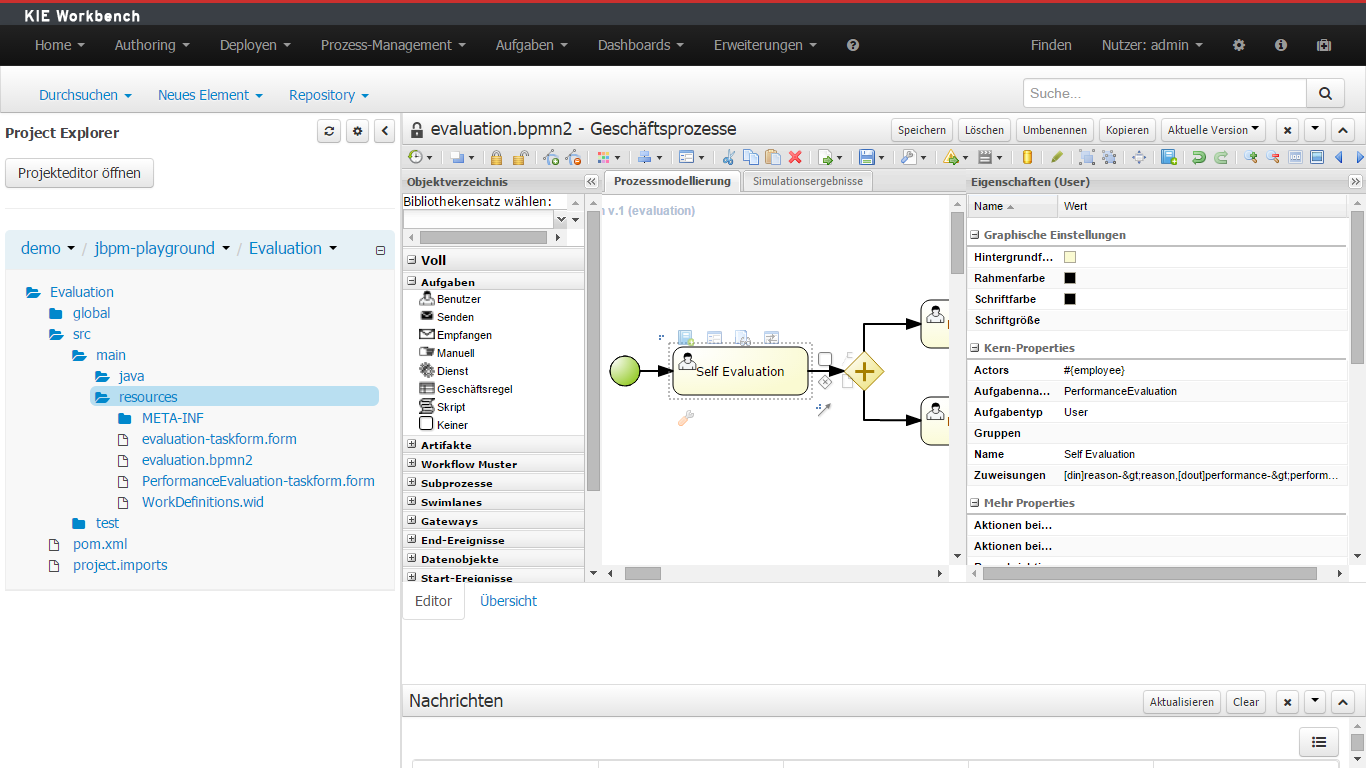
\includegraphics[width=0.95\linewidth]{../Bilder/KieWorkbench}
\caption{KIE Workbench Prozessdesigner}
\label{fig:KieWorkbench}
\end{figure}

\subsection{Eclipse BPMN 2.0 Modeler}
Der BPMN 2.0 Modeler ist ein Plugin für die Eclipse Entwicklungsumgebung. Das Plugin ermöglicht eine intuitive und komfortable Gestaltung von Geschäftsprozessen. Dabei müssen Prozessschritte, die eine Interaktion mit dem Endanwender erfordern, als Workitemhandler in Java implementiert werden. Um den Prozess starten zu können muss eine KIE Runtime angelegt und eine KIE Session instantiiert werden. Dabei ermöglicht uns die Kombination aus Entwicklungsumgebung und Debugger mehr Kontrolle über die Geschehnisse. Aufgrund der Zuverlässigkeit des Designers und trotz der Mehraufwände besonders durch die eigene Implementierung einer grafischen Benutzerschnittstelle, war die Wahl des BPMN Modeler und die Umsetzung in Eclipse die bessere Entscheidung. 